\documentclass[12pt,a4paper]{report}
\usepackage[utf8]{inputenc}
\usepackage{amsmath}
\usepackage{amsfonts}
\usepackage{amssymb}
\usepackage{amsthm}
\usepackage{hyperref}

\usepackage{multicol}
\usepackage{fancyhdr}
\usepackage[inline]{enumitem}
\usepackage{tikz}
\usepackage{tikz-cd}
\usetikzlibrary{calc}
\usetikzlibrary{shapes.geometric}
\usetikzlibrary{positioning}
\usepackage[margin=0.5in]{geometry}
\usepackage{xcolor}

\hypersetup{
    colorlinks=true,
    linkcolor=blue,
    filecolor=magenta,      
    urlcolor=cyan,
    pdftitle={Tensors},
    pdfpagemode=FullScreen,
    }

%\urlstyle{same}

\newcommand{\CLASSNAME}{Math 5050 -- Special Topics: Differential Geometry}
\newcommand{\STUDENTNAME}{Paul Carmody}
\newcommand{\ASSIGNMENT}{Section 14: Vector Fields }
\newcommand{\DUEDATE}{October 8, 2025}
\newcommand{\PROFESSOR}{Professor Berchenko-Kogan}
\newcommand{\SEMESTER}{Fall 2025}
\newcommand{\SCHEDULE}{TBD}
\newcommand{\ROOM}{Remote}

\newcommand{\MMN}{M_{m\times n}}
\newcommand{\FF}{\mathcal{F}}

\pagestyle{fancy}
\fancyhf{}
\chead{ \fancyplain{}{\CLASSNAME} }
%\chead{ \fancyplain{}{\STUDENTNAME} }
\rhead{\thepage}
\input{../MyMacros}

\newcommand{\RED}[1]{\textcolor{red}{#1}}
\newcommand{\BLUE}[1]{\textcolor{blue}{#1}}

\newcommand{\SUPP}{\operatorname{supp}}
\newcommand{\CLOSURE}{\operatorname{closure of}}

\begin{document}

\begin{center}
	\Large{\CLASSNAME -- \SEMESTER} \\
	\large{ w/\PROFESSOR}
\end{center}
\begin{center}
	\STUDENTNAME \\
	\ASSIGNMENT -- \DUEDATE\\
\end{center} 

\textbf{\Large{Notes:}}
	
\textbf{Exercises}

\HLINE
\begin{enumerate}[label=14.\arabic*]

	\item \textbf{Equality of vector fields}
	
	Show that two $C^\infty$ vector fields $X$ and $Y$ on a manifold $M$ are equal if and only if for every $C^\infty$ function $f$ on $M$, were have $Xf = Yf$.
	\BLUE{\begin{description}
		\item $(\Rightarrow)$ Since $X = Y$ a single basis can be used for both.  Thus, the differentials will be the same.
		\item $(\Leftarrow)$ Assume that $Xf = Yf$ for all $f$ on $M$.\\
		For any chart $(U, x_1, \dots, x_n)$ we have 
		\begin{align*}
			XF &= \sum_{i=1}^n X^i\PART{f}{x^i} \AND YF = \sum_{i=1}^n Y^i\PART{f}{x^i}\\
			\sum_{i=1}^n X^i\PART{f}{x^i} &= \sum_{i=1}^n Y^i\PART{f}{x^i}\\
			0 &= \sum_{i=1}^n X^i\PART{f}{x^i} - \sum_{i=1}^n Y^i\PART{f}{x^i}\\
			&= \sum_{i=1}^n X^i\PART{f}{x^i} - Y^i\PART{f}{x^i}\\
			&= \sum_{i=1}^n (X^i - Y^i)\PART{f}{x^i}\\
		\end{align*}Since $f$ represents ANY function this must be true even when $\PART{f}{x^i} \ne 0$ for all $i=1, \dots, n$.  Therefore, $X^i=Y^i$.  Since $(U, x^1,\dots, x^n)$ was also arbitrary, $X=Y$.
\end{description}	
	}
	
	\item \textbf{Vector field on an odd sphere}
	
	Let $x^1,y^1, \dots, x^n,y^n$ be the standard coordinates on $\R^{2n}$.  The unit sphere $S^{2n-1}$ in $\R^{2n}$ is defined by the equation $\SUM{i=1}{n} (x^i)^2+(y^i)^2=1$. Show that
	\begin{align*}
		X = \sum_{i=1}^n -y^i\PART{}{x^i}+x^i\PART{}{y^i}
	\end{align*}is a nowhere-vanishing smooth vector field on $S^{2n-1}$.  Since all spheres of the same dimension are diffeomorphic, this proves that on every odd-dimensional sphere there is nowhere vanishing smooth vector field.  It is a classical theorem of differential and algebraic topology that on an even-dimensional sphere every continuous vector field must vanish somewhere.
	
	\BLUE{Need to show that $X_p\ne 0$ for all $p \in S^{2n-1}$, where 
	\begin{align*}
		f(x^1,y^1, \dots, x^n,y^n) &= \SUM{i=1}{n} (x^i)^2+(y^i)^2-1
	\end{align*}so given a point $p=(x^1,y^1, \dots, x^n,y^n)$ then
	\begin{align*}
		\RBAR{\PART{f}{x^j}}_p &= 2x^j \AND \RBAR{\PART{f}{y^i}}_p = 2y^j \\
		X_p &= \sum_{i=1}^n -y^i\RBAR{\PART{}{x^i}}_p+x^i\RBAR{\PART{}{y^i}}_p \\
		\therefore X_p(f) &= \sum_{j=1}^n \PAREN{-y^j2x^j+x^j 2y^j} \\
		&= 0.
	\end{align*}But, for $X$ to vanish $(x^1,-y^1, x^2,-y^2, \dots, x^n, -y^n)=0$ which only happens at the origin.  This point is not a solution for $\sum_{i=1}^n (x^i)^2+(y^i)^2 = 1$ and is not on the sphere.
	}
	
	\item \textbf{Maximal integral curve on a punctured line}
	
	Let $M$ be $\R-\{0\}$ and let $X$ be the vector field $d/dx$ on $M$ (Figure 14.3).  Find the maximal integral curve of $X$ starting at $x=1$.
	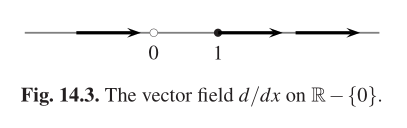
\includegraphics[scale=0.5]{14_3.png} 
	
	\item \textbf{Integral curves in the plane}
	
	Find the integral curves of the vector field 
	\begin{align*}
		X_{(x,y)} &= x\PART{}{x}-y\PART{}{y} = \SQCOLVECTOR{x \\ -y} \, \text{ on } \R^2.
	\end{align*}
	
	\item \textbf{Maximal integral curve in the plane}
	
	Find the maximal integral curve $c(t)$ starting at the point $(a,b)\in \R^2$ of the vector field $X_{(x,y)} = \PART{}{x}+x\PART{}{y}$ on $\R^2$.
	
	\item \textbf{Integral curve starting at a zero of a vector field}
	
	\begin{enumerate}[label=(\alph*)]
	
		\item Suppose the smooth vector field $X$ on a manifold $M$ vanishes at a point $p \in M$.  Show that the integral curve of $X$ with initial point $p$ is the constant curve $c(t) \equiv p$.
		
		\item Show that if $X$ is the zero vector field on a manifold $M$, and $c_t(p)$ is the maximal integral curve of $X$ starting at $p$, then the one-parameter group of diffeomorphisms $c: \R\to \operatorname{Diff}(M)$ is the constant map $c(t) \equiv \mathbf{I}_m$
	
	\end{enumerate}
	
	\item \textbf{Maximal integral curve}
	
	Let $X$ be the vector field $xd/dx$ on $\R$.  For each $p$ in $\R$, find the maximal integral curve $c(t)$ of $X$ starting at $p$.
	
	\item \textbf{Maximal integral curve}
	
	Let $X$ be the vector field $x^2 d/dx$ on the real line $\R$.  For each $p > 0$ in $\R$, find the maximal integral curve of $X$ with initial point $p$.
	
	\item \textbf{Reparametrization of a integral curve}
	
	Suppose $c:(a,b)\to M$ is an integral curve of the smooth vector field $X$ on $M$.  Show that for any real number $s$, the map
	\begin{align*}
		c_s: (a+x, b+x)\to M, \, c_s(t)=c(t-2)
	\end{align*}is also an integral curve of $X$.
	
	\item \textbf{Lie bracket of vector fields}
	
	If $f$ and $g$ are $C^\infty$ functions and $X$ and $Y$ are $C^\infty$ vector fields on a manifold $M$, show that 
	\begin{align*}
		[fX,gY] = fg[X,Y]+f(Xg)Y-g(Yf)X.
	\end{align*}
	
	\BLUE{Remember that the Lie Bracket on vector fields is
	\begin{align*}
		[X,Y] &= XY-YX 
	\end{align*}So,
	\begin{align*}
		[fX,gY] &= (fX)(gY) - (gY)(fX) \\
		&= T_1 - T_2 
	\end{align*}We must keep in mind that these are operators executed on some function $h$.  Thus,
	\begin{align*}
		T_1(h) &= (fX)(gY)(h)\\
		&= f\cdot\PAREN{(Xg)Y(h)+g(XY)(h)} \\
		&= f(Xg)Y(h)+fg(XY)(h)
	\end{align*}similarly
	\begin{align*}
		T_2(h) &= (gY)(fX)(h) \\
		&= g\cdot\PAREN{(Yf)X(h)+f(YX)(h)} \\
		&= g(Yf)X(h)+gf(YX)(h)
	\end{align*}then
	\begin{align*}
		T_1 - T_2 &= f(Xg)Y(h)+fg(XY)(h) - (g(Yf)X(h)+gf(YX)(h)) \\
		&= fg[X,Y](h) + f(Xg)Y(h) - g(Yf)X(h)
	\end{align*}
	}
	
	\item \textbf{Lie bracket of vector fields on $\R^2$}
	
	Compute the Lie bracket
	\begin{align*}
		\SQBRACKET{-y\PART{}{x}+x\PART{}{y}, \PART{}{x}}
	\end{align*}on $\R^2$.
	
	\BLUE{
	\begin{align*}
		\SQBRACKET{-y\PART{}{x}+x\PART{}{y}, \PART{}{x}} &= \PAREN{-y\PART{}{x}+x\PART{}{y}}\PAREN{\PART{}{x}}-\PAREN{\PART{}{x}}\PAREN{-y\PART{}{x}+x\PART{}{y}} \\
		&= -y\frac{\partial^2}{\partial^2 x} + x\frac{\partial ^2}{\partial y\partial x} - \PAREN{-y\frac{\partial^2}{\partial^2 x} + \PART{}{y}+x\frac{\partial^2}{\partial x\partial y}} \\
		&= \PART{}{y}
	\end{align*}
	}
	
	\item \textbf{Lie bracket in local coordinates}
	
	Consider two $C^\infty$ vector fields, $X, Y$ on $\R^n$:
	\begin{align*}
		X = \sum a^i\PART{}{x^i}, \, Y=\sum b^j\PART{}{x^j}
	\end{align*}for some $C^\infty$ function $c^k$.  Find the formula for $c^k$ in terms of $a^i$ and $b^i$.
	
	\item \textbf{Vector field under a diffeomorphism}
	
	Let $F: N \to M$ be a $C^\infty$ diffeomorphism of manifolds.  Prove that if $g$ is a $C^\infty$ function and $X$ a $C^\infty$ vector field on $N$, then
	\begin{align*}
		F_*(gX) = (g\circ F^{-1})F_*X.
	\end{align*}
	
	\item \textbf{Lie bracket under a differomorphism}
	
	Let $F: N \to M$ be a $C^\infty$ diffeomorphism of manifolds.  Prove that if $X$ and $Y$ are $C^\infty$ vector fields  on $N$, then 
	\begin{align*}
		F_*[X,Y]=[F_*X, F_*Y].
	\end{align*}
\end{enumerate}

\end{document}
